\section{Datapath Optimization} \label{sec:dtptopti}
\subsection{Systolic Arrays}
Systolic arrays were implemented on the first \acrshort{fpga}-based accelerators. A static systolic array is a static array of \acrshort{pe} doing a part of the computation and communicating with its neighbors. An illustration of its principle can be found on figure \ref{fig:sytar}. The configuration can only support convolution with a kernel size $K_*$ lower than a bound, such that $K_* \leq K_m$. The systolic array allows spatial data reutilisation between rows and columns and temporal data reutilisation.\newline \newline
\begin{figure}
    \centering
    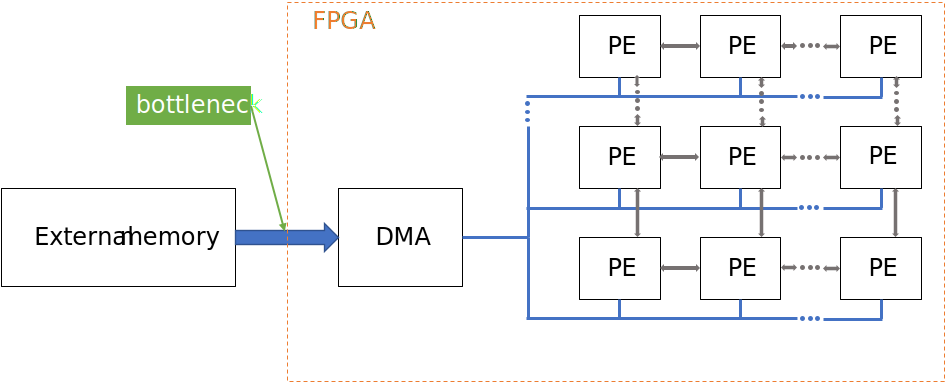
\includegraphics[width=\textwidth]{systArray.pdf}
    \label{fig:sytar}
    \caption{Static Systolic Arrays}
\end{figure}
However, Systolic Arrays has also issues. First, when the kernel size is much lesser than the maximal kernel size ($K_* << K_m$), there is an underutilization of the resources. For example, \cite{gokhale_240_2014} notes that for a $3 \times 3$ kernel, only $9\%$ of the \acrfull{dsp} blocks are used. Second,  data caching is not implemented. It means that it has always to fetch input from the external memory. Memory becomes the bottleneck and the performance is bounded by the device memory bandwidth.
\subsection{Data-flow \acrshort{moc} for \acrshort{cnn}s}
Data-flow \acrfull{moc} can be used to accelerate \acrshort{cnn}s on \acrshort{fpga}. This approach is motivated because the feed-forward aspect of the inference stage of the \acrshort{cnn} is purely data driven.
Data-flow \acrfull{moc} were firstly investigated by \cite{lin_li_low_2016}.  We describe the \acrshort{cnn} as a network where:
\begin{itemize}
    \item \textbf{nodes} are processing unit called an \textit{actor}. Each actor follows a data-driven exectution where the execution is triggered by the availability of input, which is the case for a \acrshort{cnn}.
    \item \textbf{edges} are communication \acrshort{fifo} channels. Actors exchange data called \textit{tokens} through those \acrshort{fifo} channels.
\end{itemize}
A represention of such network can be found in figure \ref{fig:moc}. \newline \newline
The \acrshort{cnn} can be therefore modeled as a topology matrix and we only have to explore those matrix components (instead of tiling and unrolling parameters of section \ref{subsec:loopopti}) to minimize latency or energy consumption. Those parameters are then used to derive \acrshort{pe} and buffer configuration. However, as pointed by \cite{abdelouahab_tactics_2017}, the direct hardware mapping of \acrshort{cnn} network means that all the computations must be unrolled, we are then bounded by the hardware resources and the size of the \acrshort{cnn}, preventing implementing this approach for deep models.
\begin{figure}
    \centering
    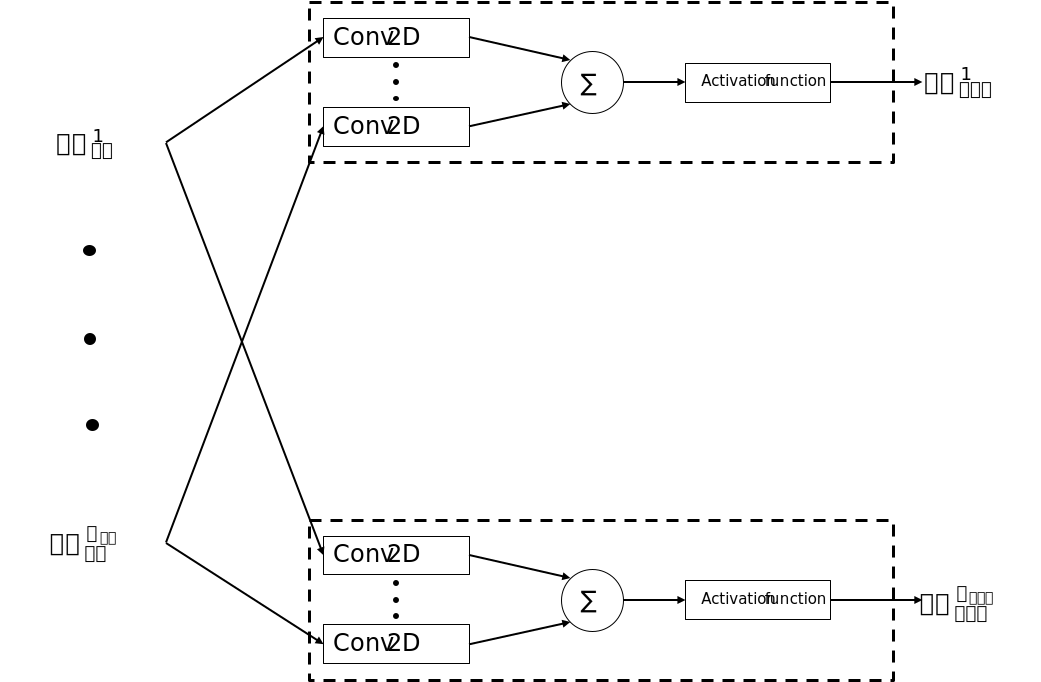
\includegraphics[width=0.8\textwidth]{Moc.pdf}
    \label{fig:moc}
    \caption{Graph represenation of a convolution layer}
\end{figure}
\subsection{Loop Optimization} \label{subsec:loopopti}
\acrfull{simd} accelerators were proposed to solve the static systolic array inefficiency. The general computation flow can be described as follow:
\begin{enumerate}
    \item Fetch \acrshort{fm}s and weights from the external memory (\acrshort{dram}) to on-chip buffer.
    \item The \acrshort{fm}s and weights are streamed into the \acrshort{pe}.
    \item 
\end{enumerate}
\subsubsection{Loop Unrolling}
\subsubsection{Loop Tiling}
\subsubsection{Loop Interchange}
\subsection{Design space exploration}
